\chapter{Software}

I det følgende afsnit beskrives systemet software vha. UML diagrammer. Afsnittet er opdelt i to dele, en del der beskæftiger sig med software tilhørende webapplikation og en del med software til dronen. 

Indledningsvis vises design overview diagrammer, disse bruges til at danne overblink over hvordan webapplikationen skal reagere på input fra bruger. Herefter vises pakkediagrammer med tilhørende beskrivelser. De pakker der vises i pakkediagrammerne består af en eller flere klasser, der med stort samspil udfører opgaver indenfor et fælles ansvarsområde. Efter pakkediagrammerne vises en række klassediagrammer, disse bruges til at vise struktur og sammenhæng mellem pakkernes forskellige klasser, eksempelvis arv.

\newpage
\section{Design overview diagrammer}

I dette afsnit vises design overview diagrammer, som bruges til at definere hvordan systemet skal reagerer på input fra bruger.

\vspace{-5pt}
\begin{figure}[H]
	\centering
	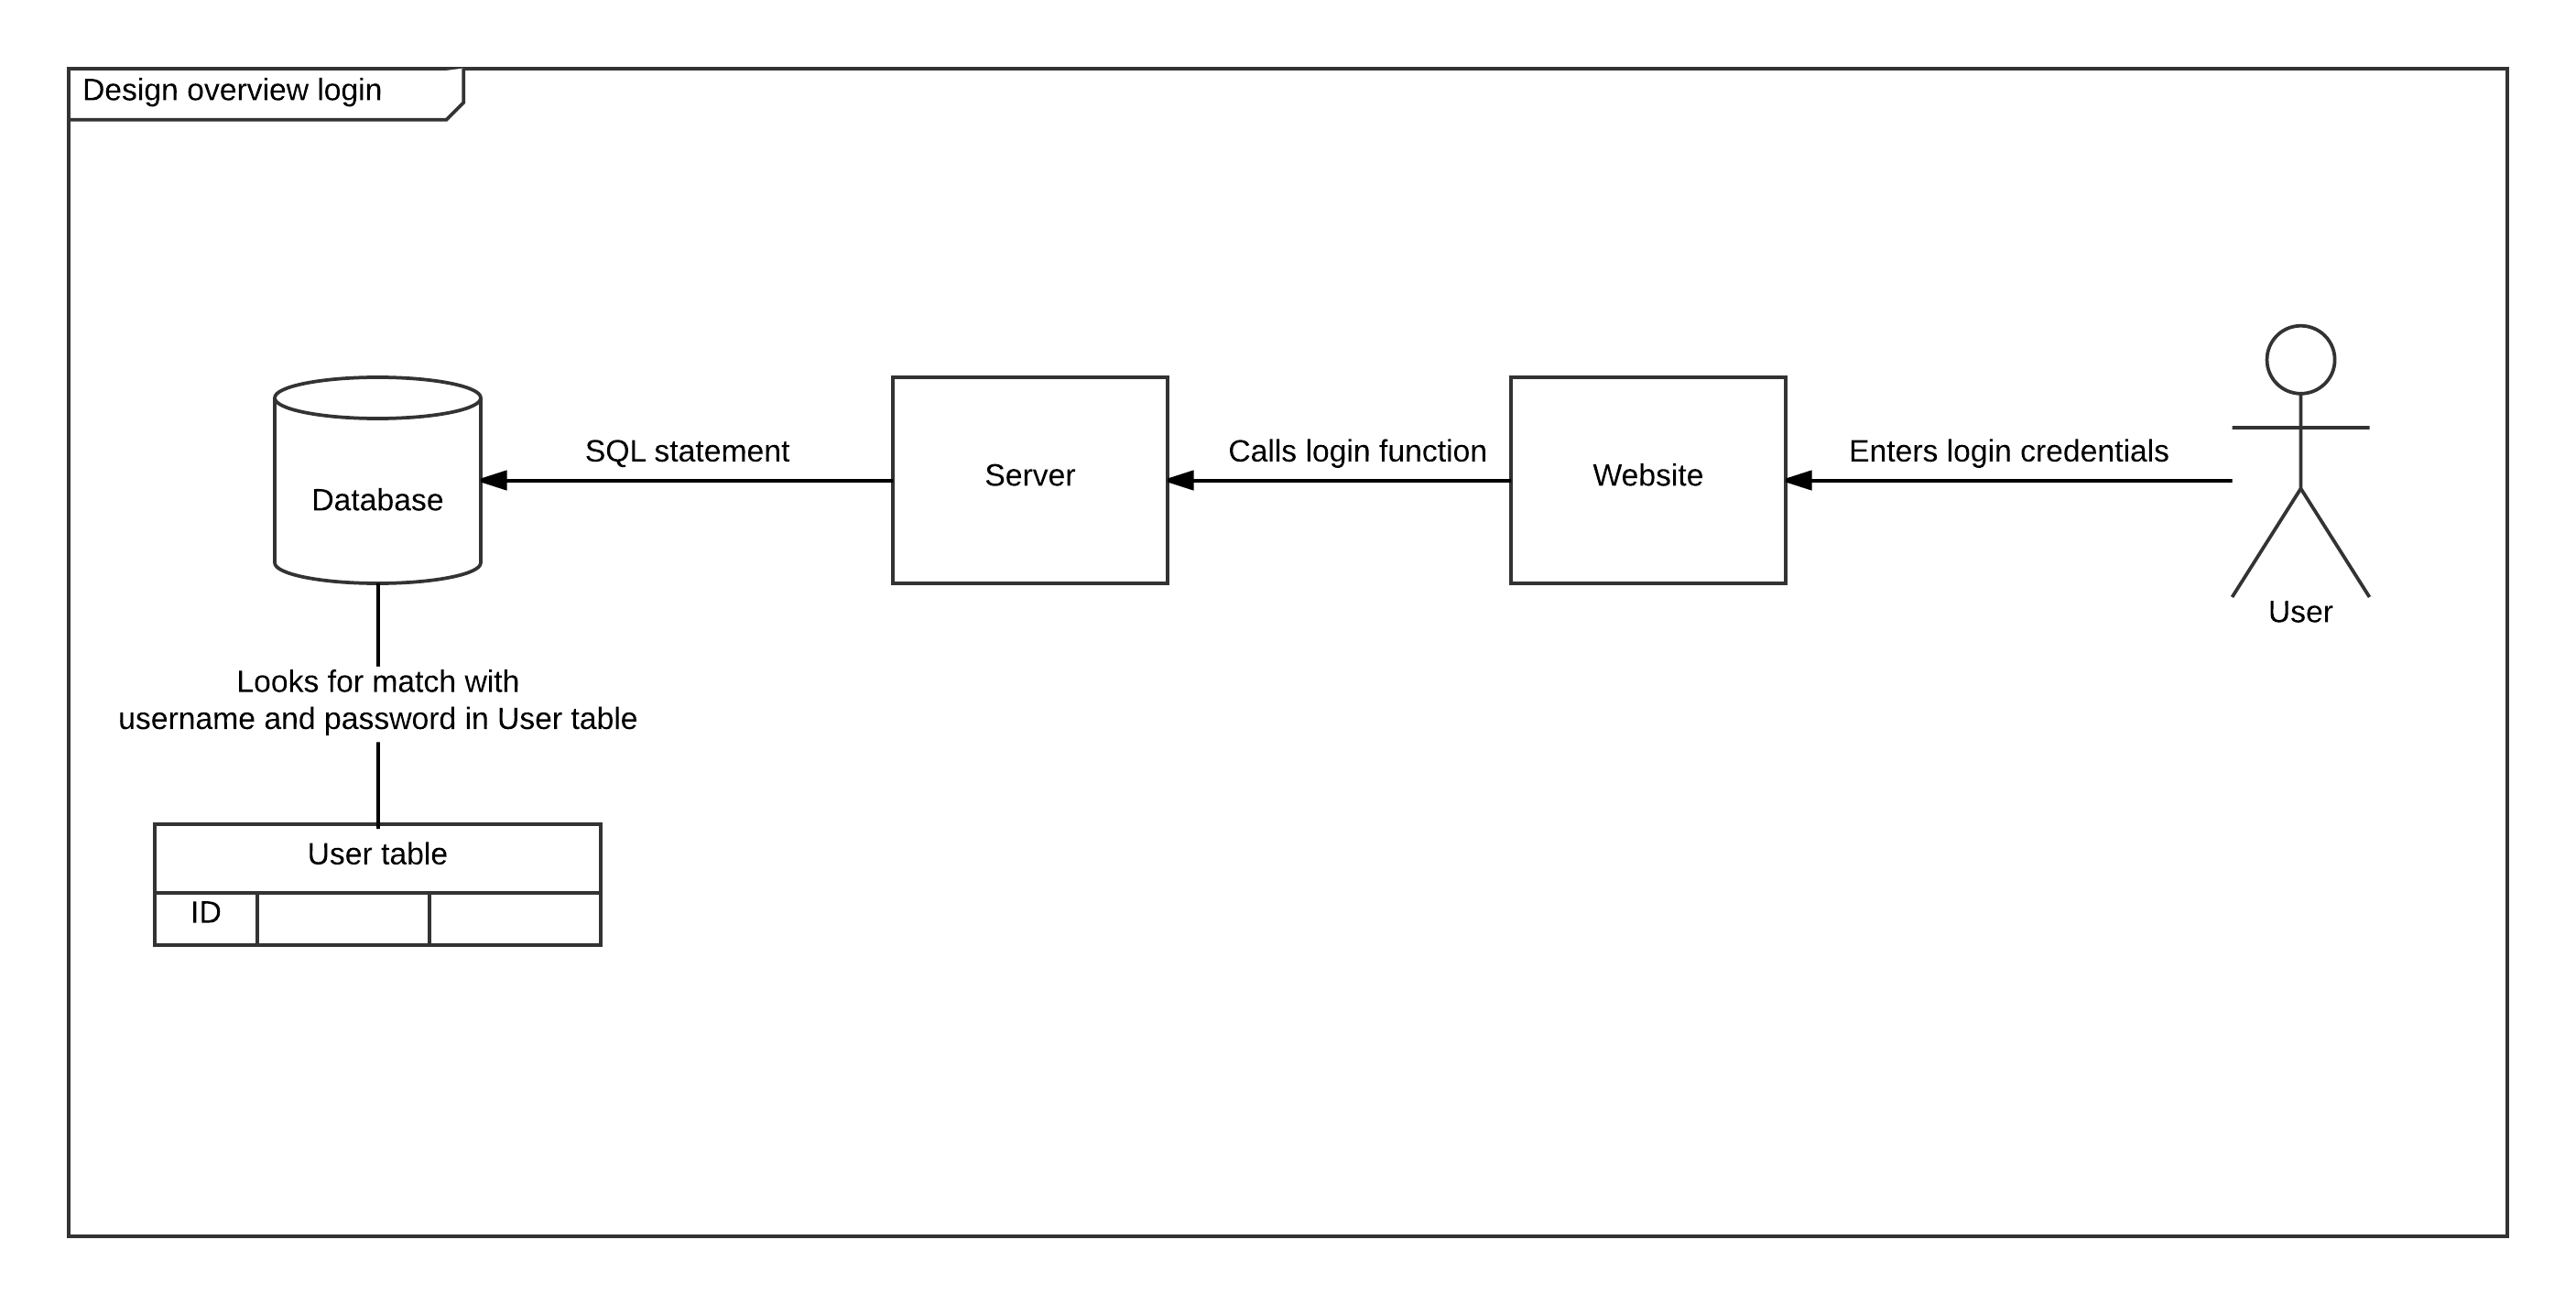
\includegraphics[width=1\textwidth]{Billeder/Design_overview/design_overview_login}
	\vspace{-1cm}
	\caption{Design overview - login}
	\label{fig:pakke_diagram}
\end{figure}

\vspace{-5pt}
\begin{figure}[H]
	\centering
	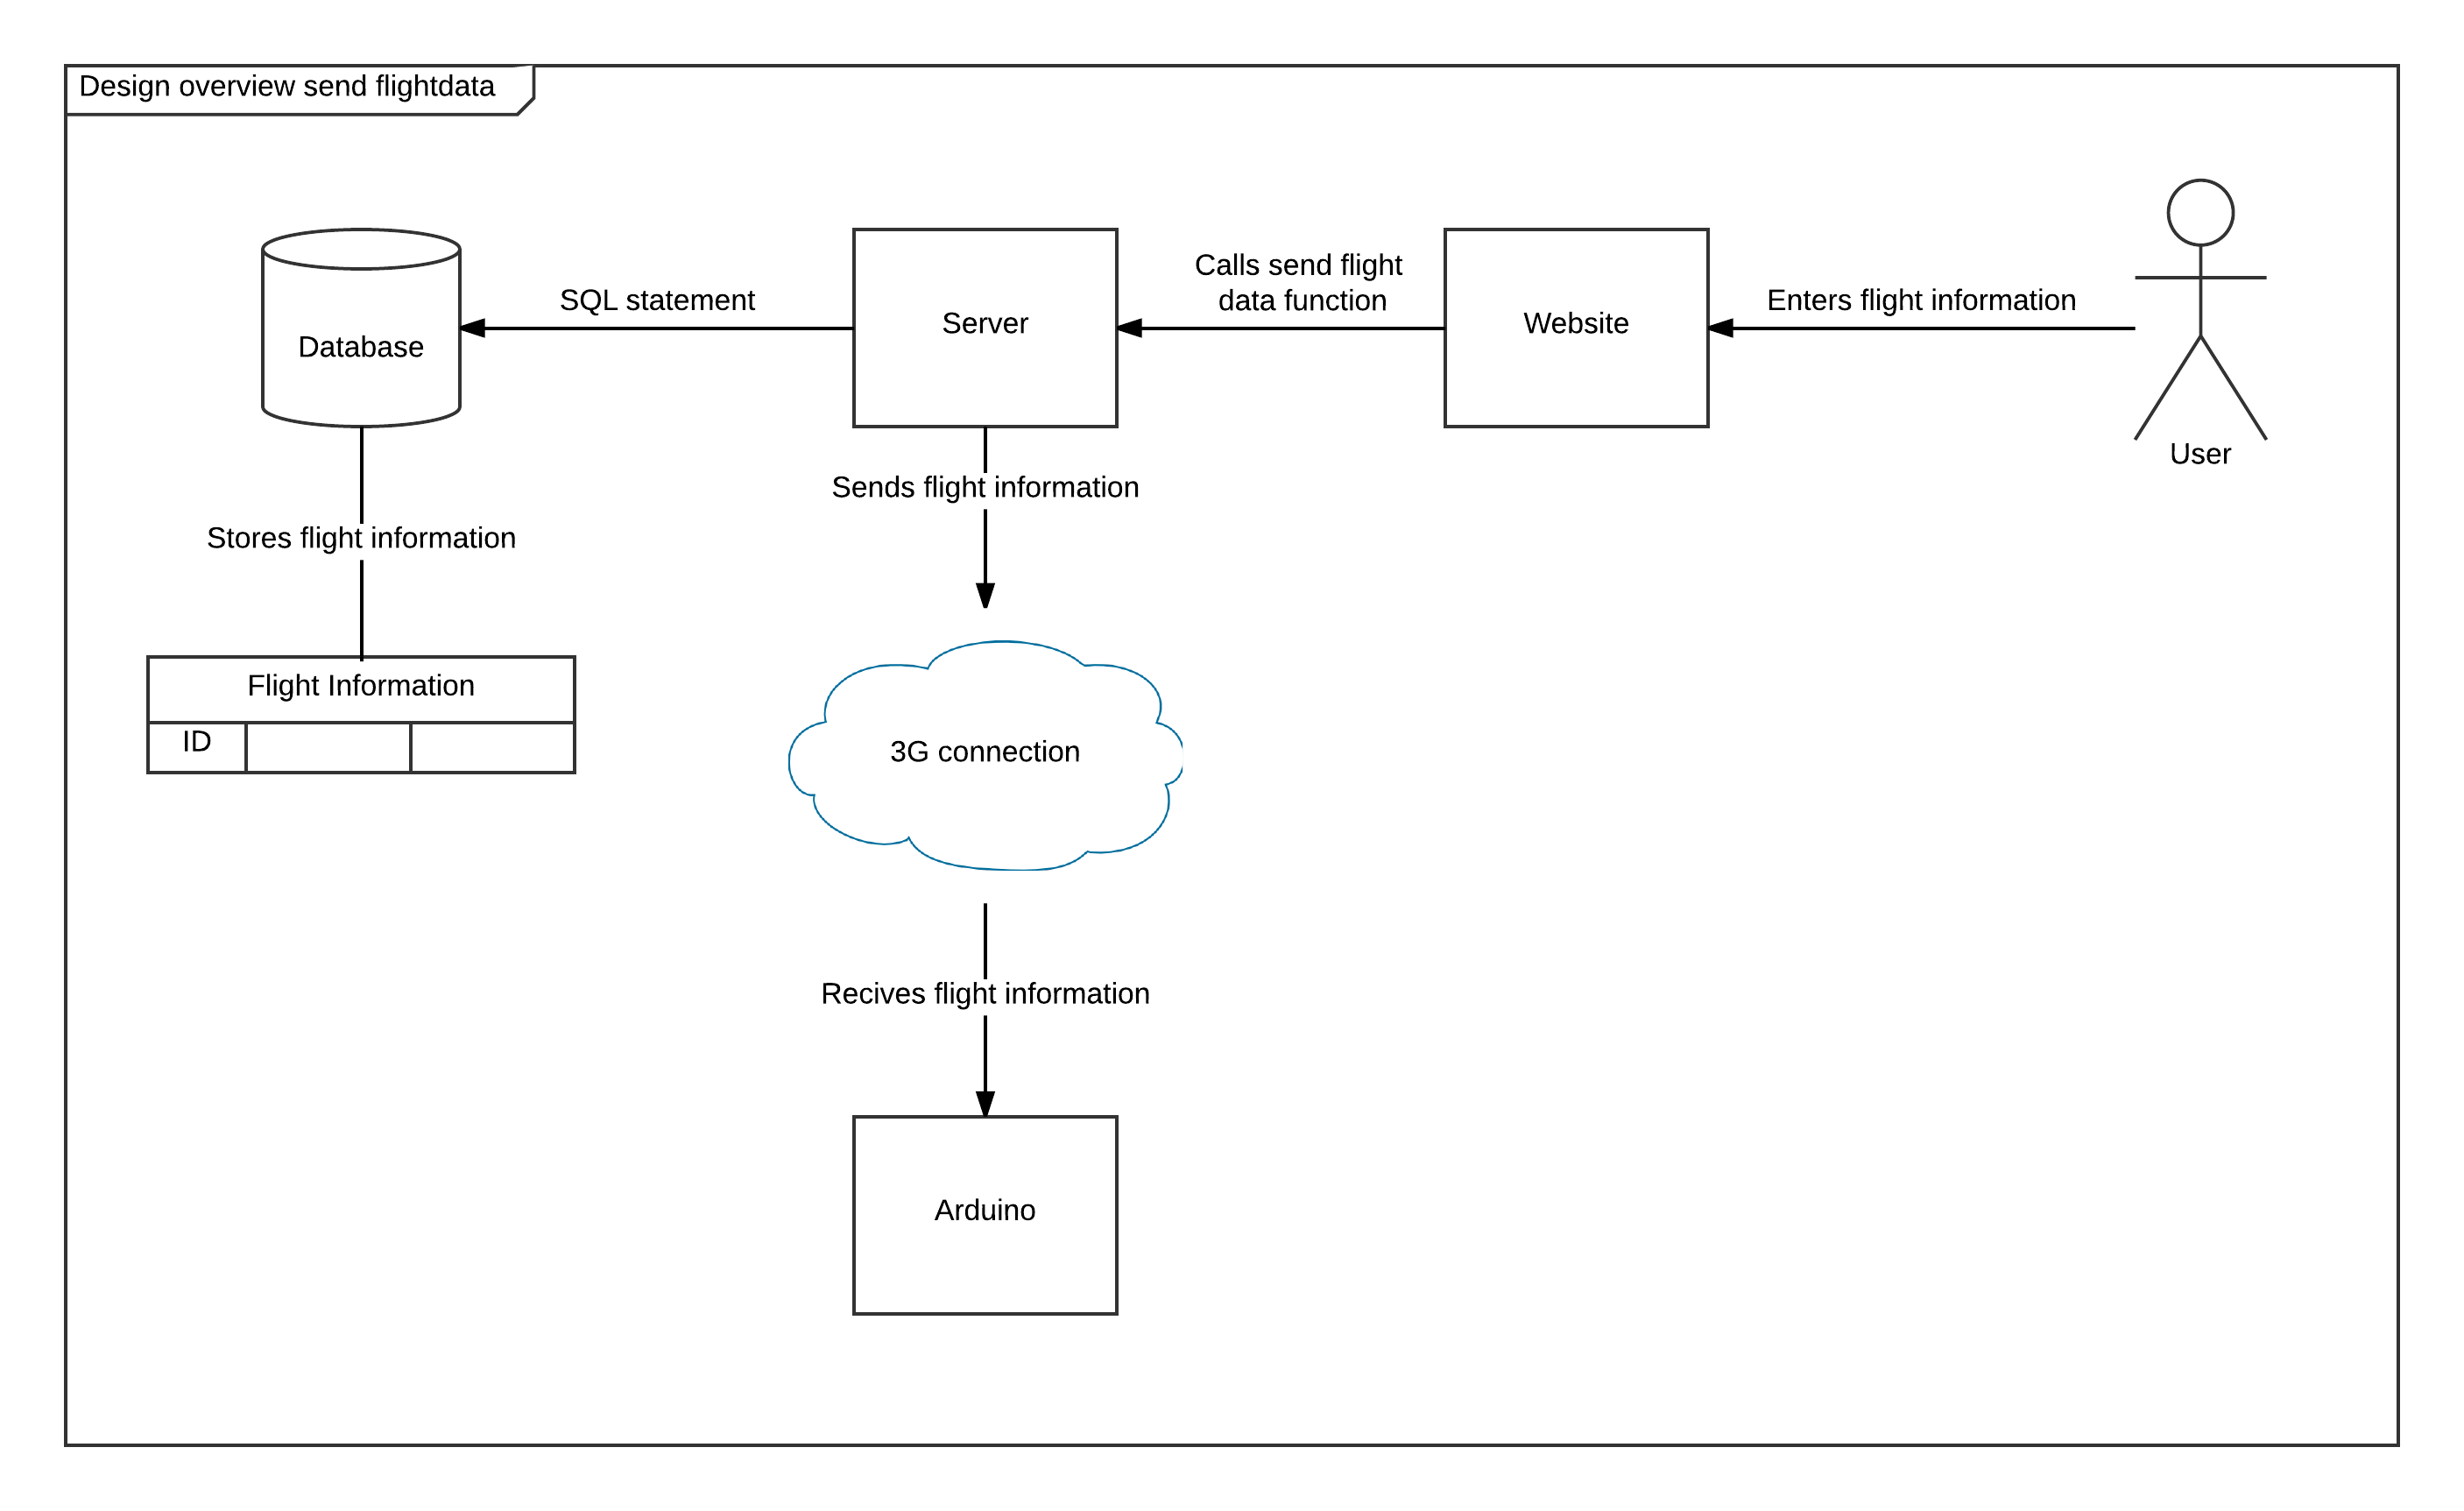
\includegraphics[width=1\textwidth]{Billeder/Design_overview/design_overview_setupFlightdata}
	\vspace{-1cm}
	\caption{Design overview - Setup fligtdata}
	\label{fig:pakke_diagram}
\end{figure}

\newpage
\section{Pakkediagram}

I denne sektion vises pakkediagrammer tilhørende webapplikation og drone. De pakker der vises i pakkediagrammerne består af en eller flere klasser, der med stort samspil udfører opgaver indenfor et fælles ansvarsområde. På hver pakke findes en lille beskrivelse, der tydeliggør pakkens ansvarsområde.

\subsection{Webapplikation}
Figur \ref{fig:pakke_diagram_webapp} viser pakkediagram over webapplikationen. 

\vspace{-5pt}
\begin{figure}[H]
	\centering
	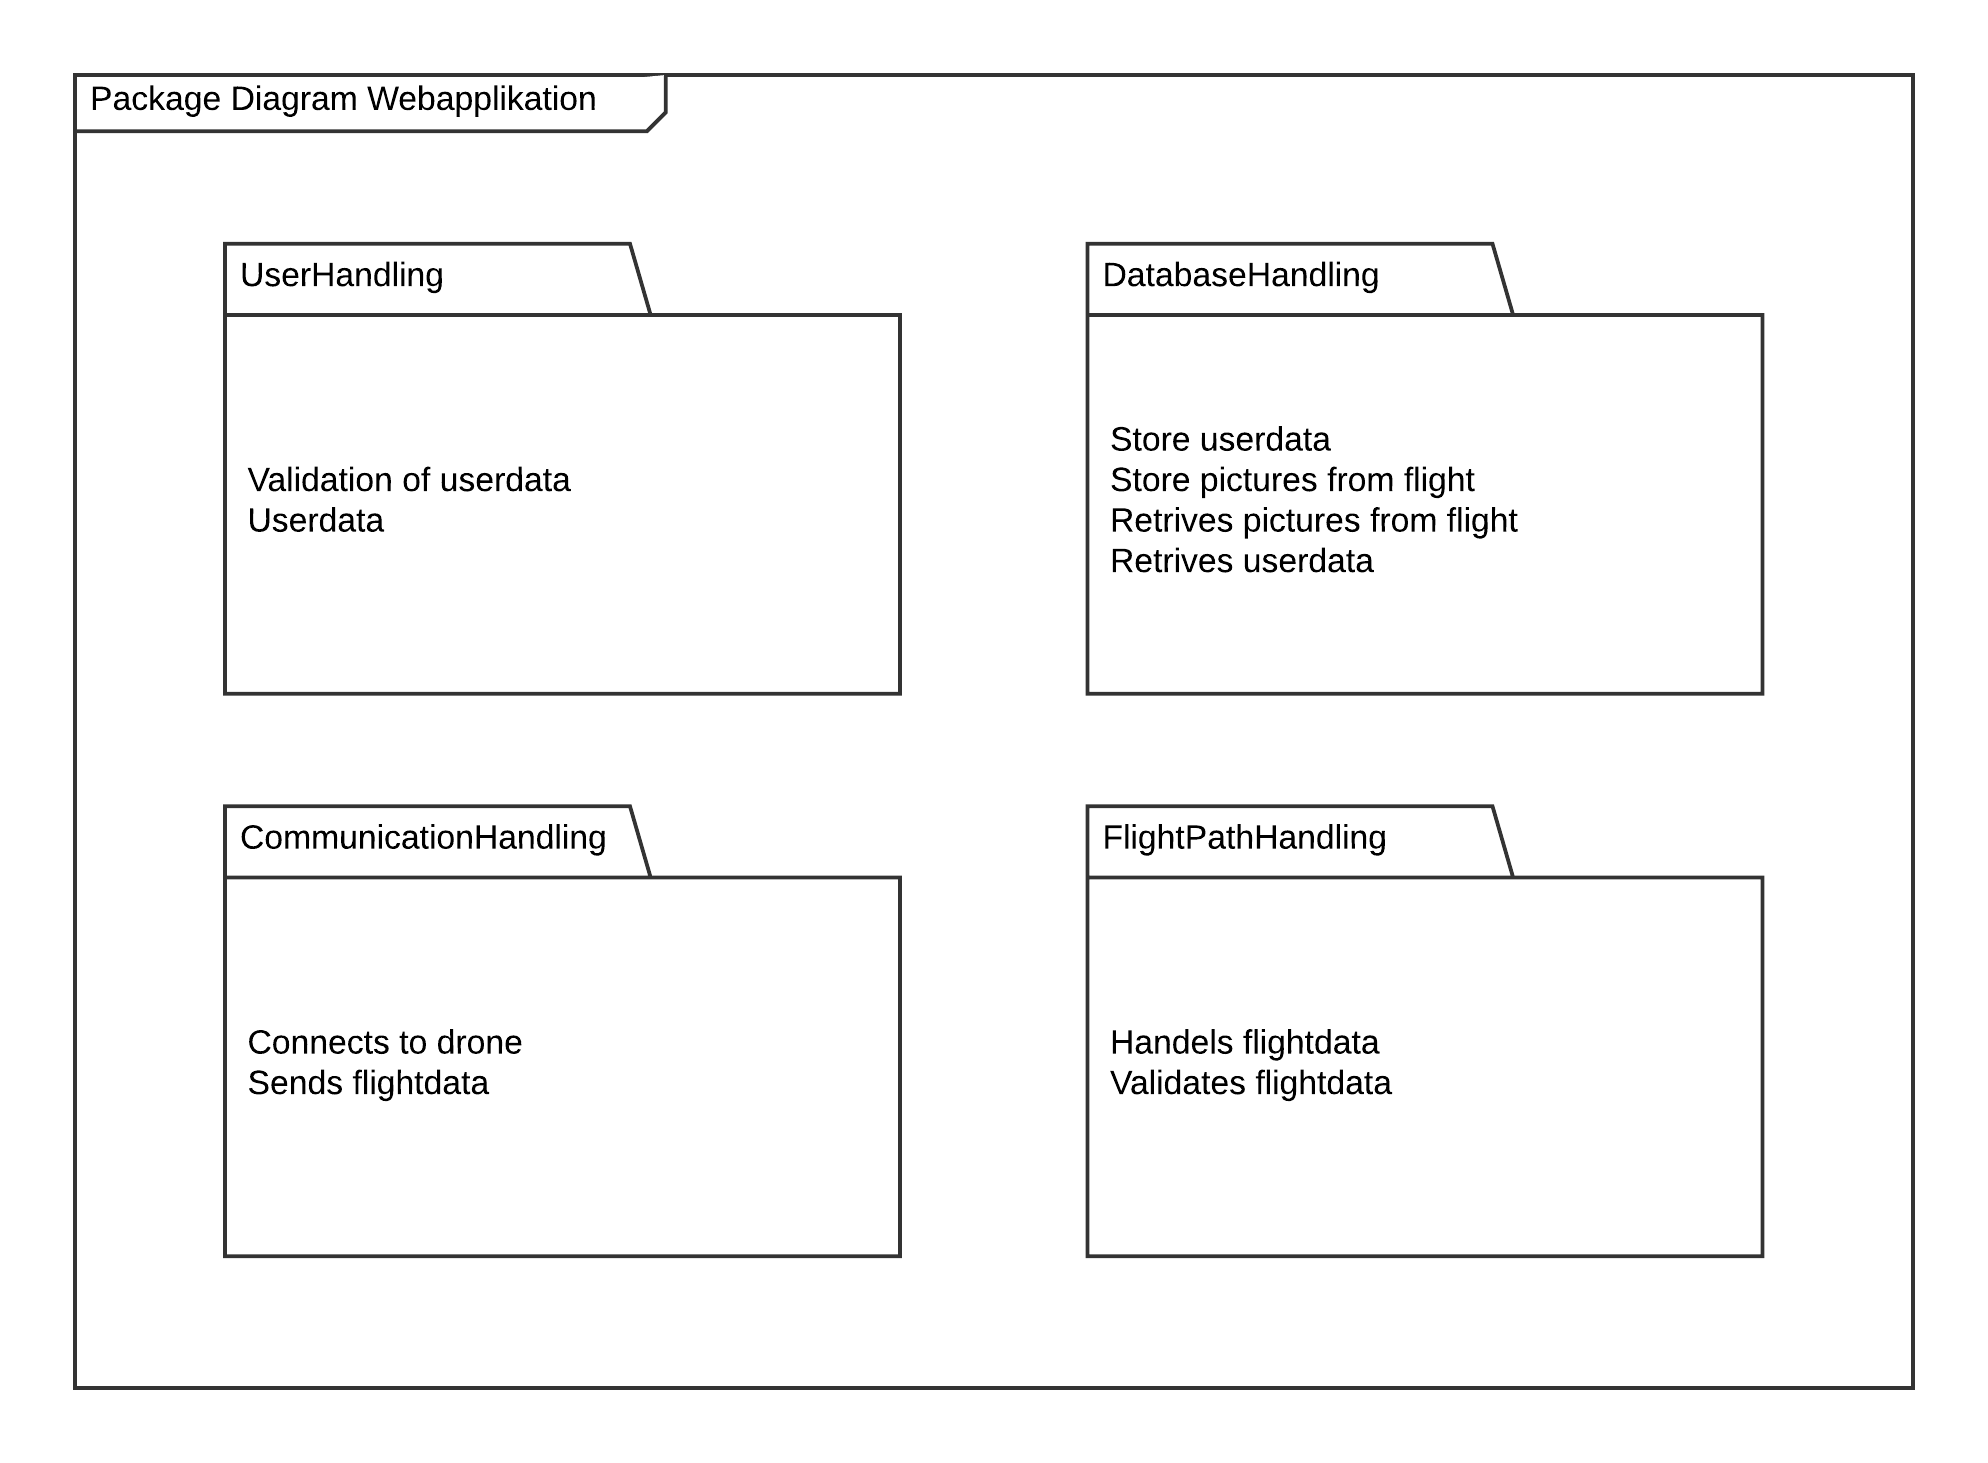
\includegraphics[width=1\textwidth]{Billeder/pakke_diagrammer/package_diagram_webapp.png}
	\vspace{-1cm}
	\caption{Overordnet pakke diagram over webapplikationen}
	\label{fig:pakke_diagram_webapp}
\end{figure}

\textbf{CommunicationHandling}\\
Pakkens ansvar er kommunikation imellem drone og server. Pakken sender flyveinformation til dronen som bruger har lavet på webapplikationen.

\textbf{UserHandling}\\
Pakkens ansvar er validering af login/log ud på websitet. Pakken har også ansvaret for at hente og gemme data om den pågældende bruger.

\textbf{DatabaseHandling}\\
Pakkens ansvar er kommunikation imellem databasen og serveren. 

\textbf{FlightPathHandling}\\
Pakkens ansvar er håndtering af flyveinformation samt validering af dataen.




\newpage
\subsection{Drone}

Figur \ref{fig:pakke_diagram_drone} viser pakkediagram over drone. 

\vspace{-5pt}
\begin{figure}[H]
	\centering
	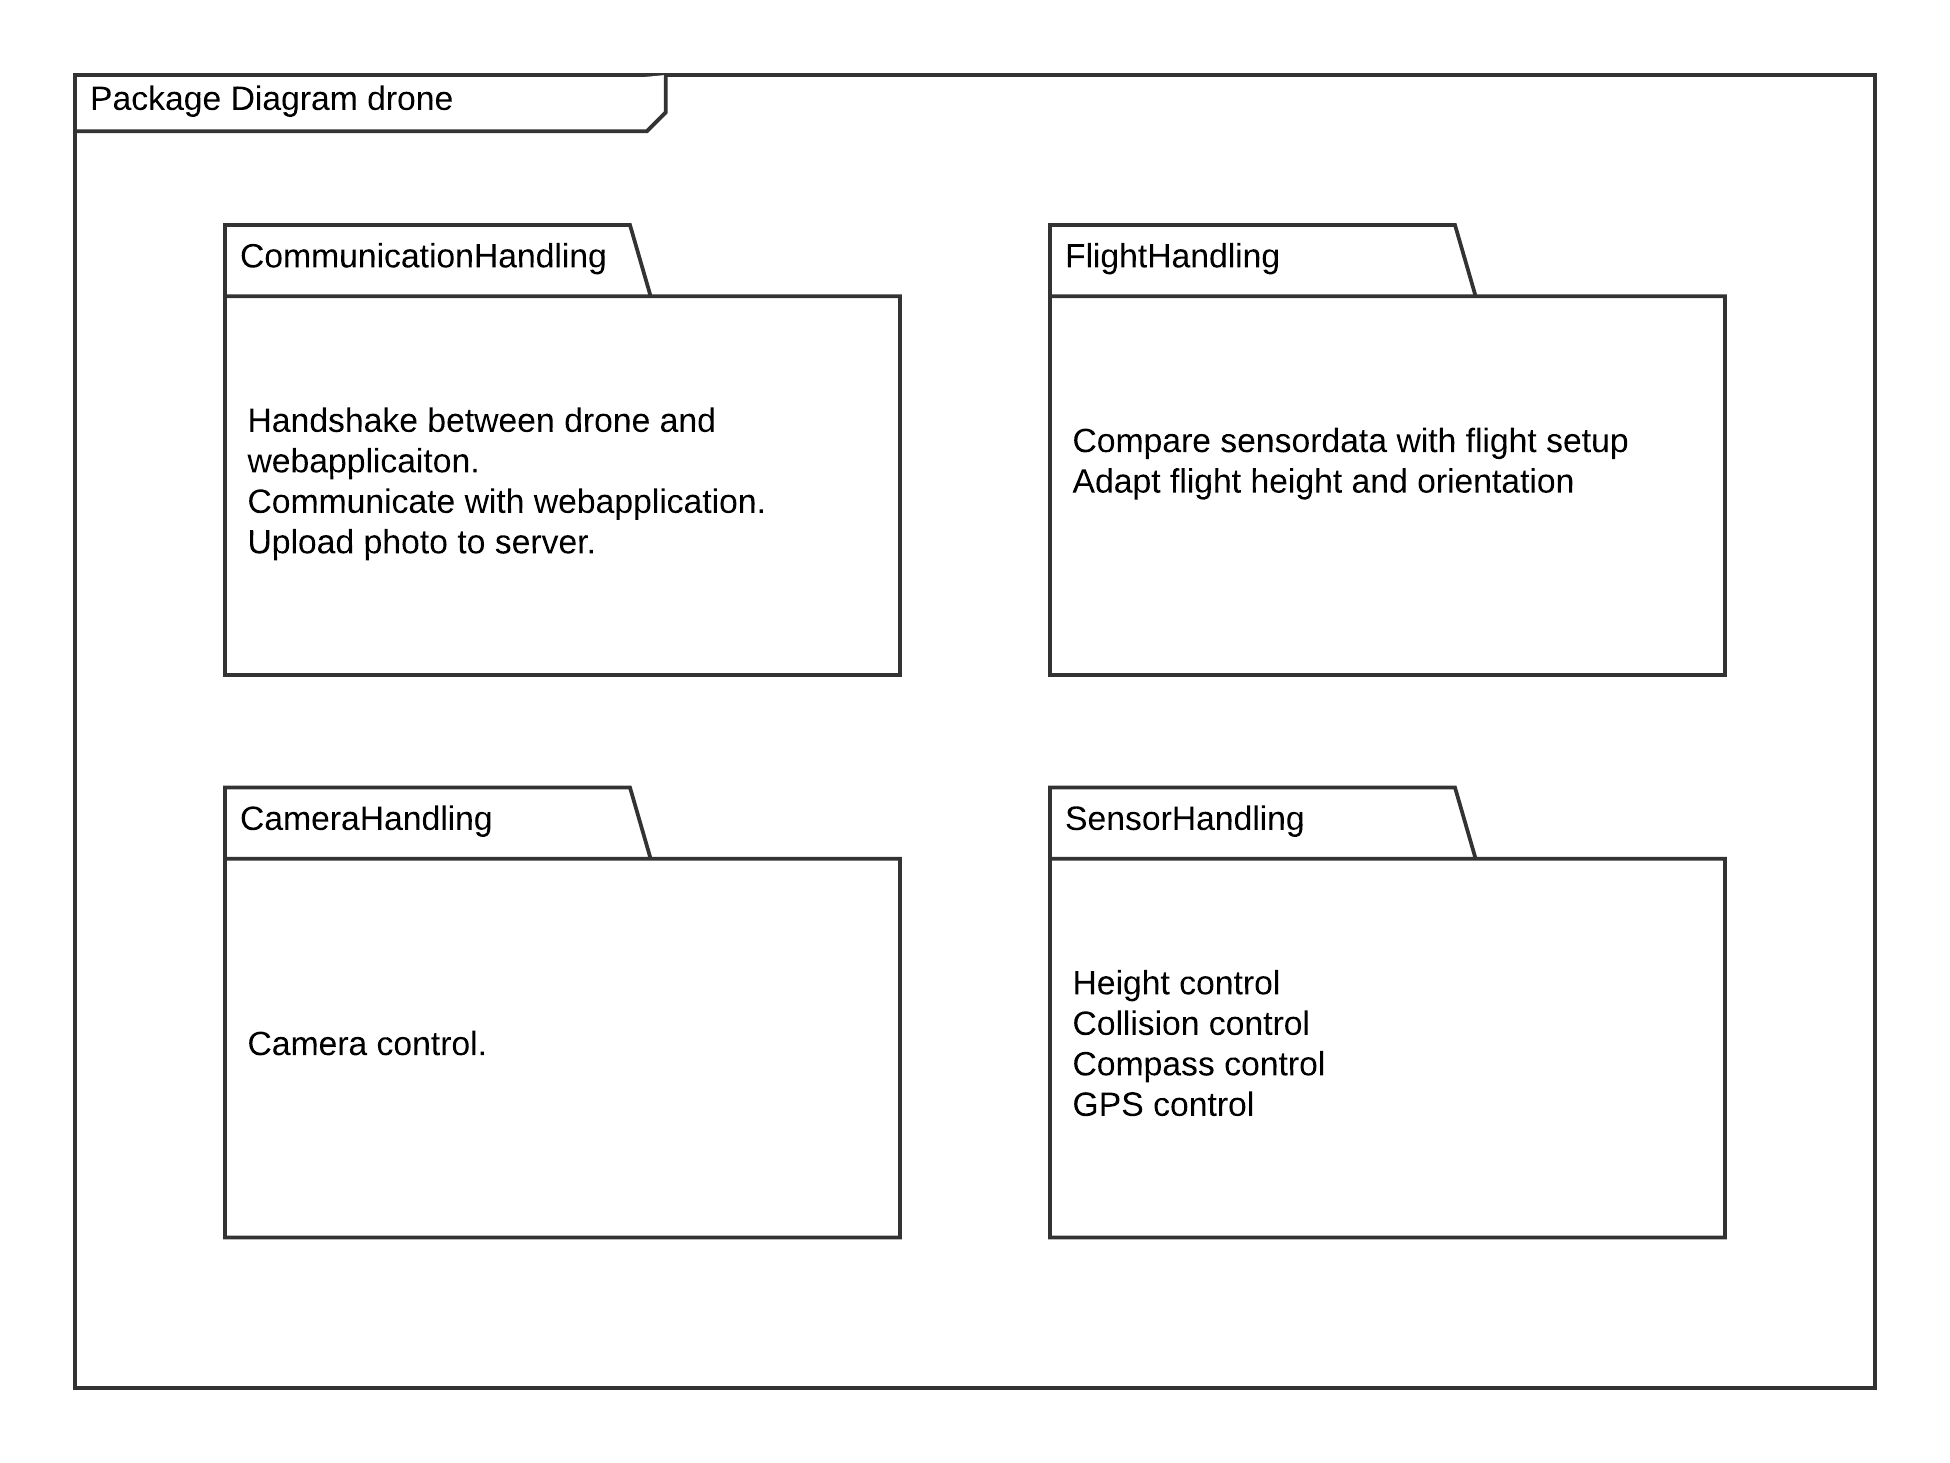
\includegraphics[width=1\textwidth]{Billeder/pakke_diagrammer/package_diagram_drone.png}
	\vspace{-1cm}
	\caption{Overordnet pakke diagram over webapplikationen}
	\label{fig:pakke_diagram_drone}
\end{figure}

\textbf{CommunicationHandling}\\
Pakkens ansvar er kommunikation imellem drone og server. Pakken modtager flyveopsætning som bruger har lavet på webapplikationen og sender billeder til webapplikation.

\textbf{FlightHandling}\\
Pakkens ansvar er at sikre dronen flyver som angivet i flyveopsætning. Pakken har til ansvar at sammenligne data fra sensorer med den modtagne flyveopsætning, og ud fra det regulere dronens flyvehøjde og orientering. 

\textbf{CameraHandling}\\
Pakkens ansvar er håndtering af kamera. Der skal kun tages billeder med kameraet når dronen er på den rette GPS position. 

\textbf{SensorHandling}\\
Pakkens ansvar er håndtering af sensor data.


\newpage
\section{Klasse diagrammer}

\subsection{FlightPathHandling klassediagram}
På klasse diagrammet FlightPathHandling ses de tre overordnet klasser hvilket udgør pakken FlightPathHandling pakken som vist på figur \ref{fig:pakke_diagram}.

\vspace{-5pt}
%kommentar
\begin{figure}[H]
	\centering
	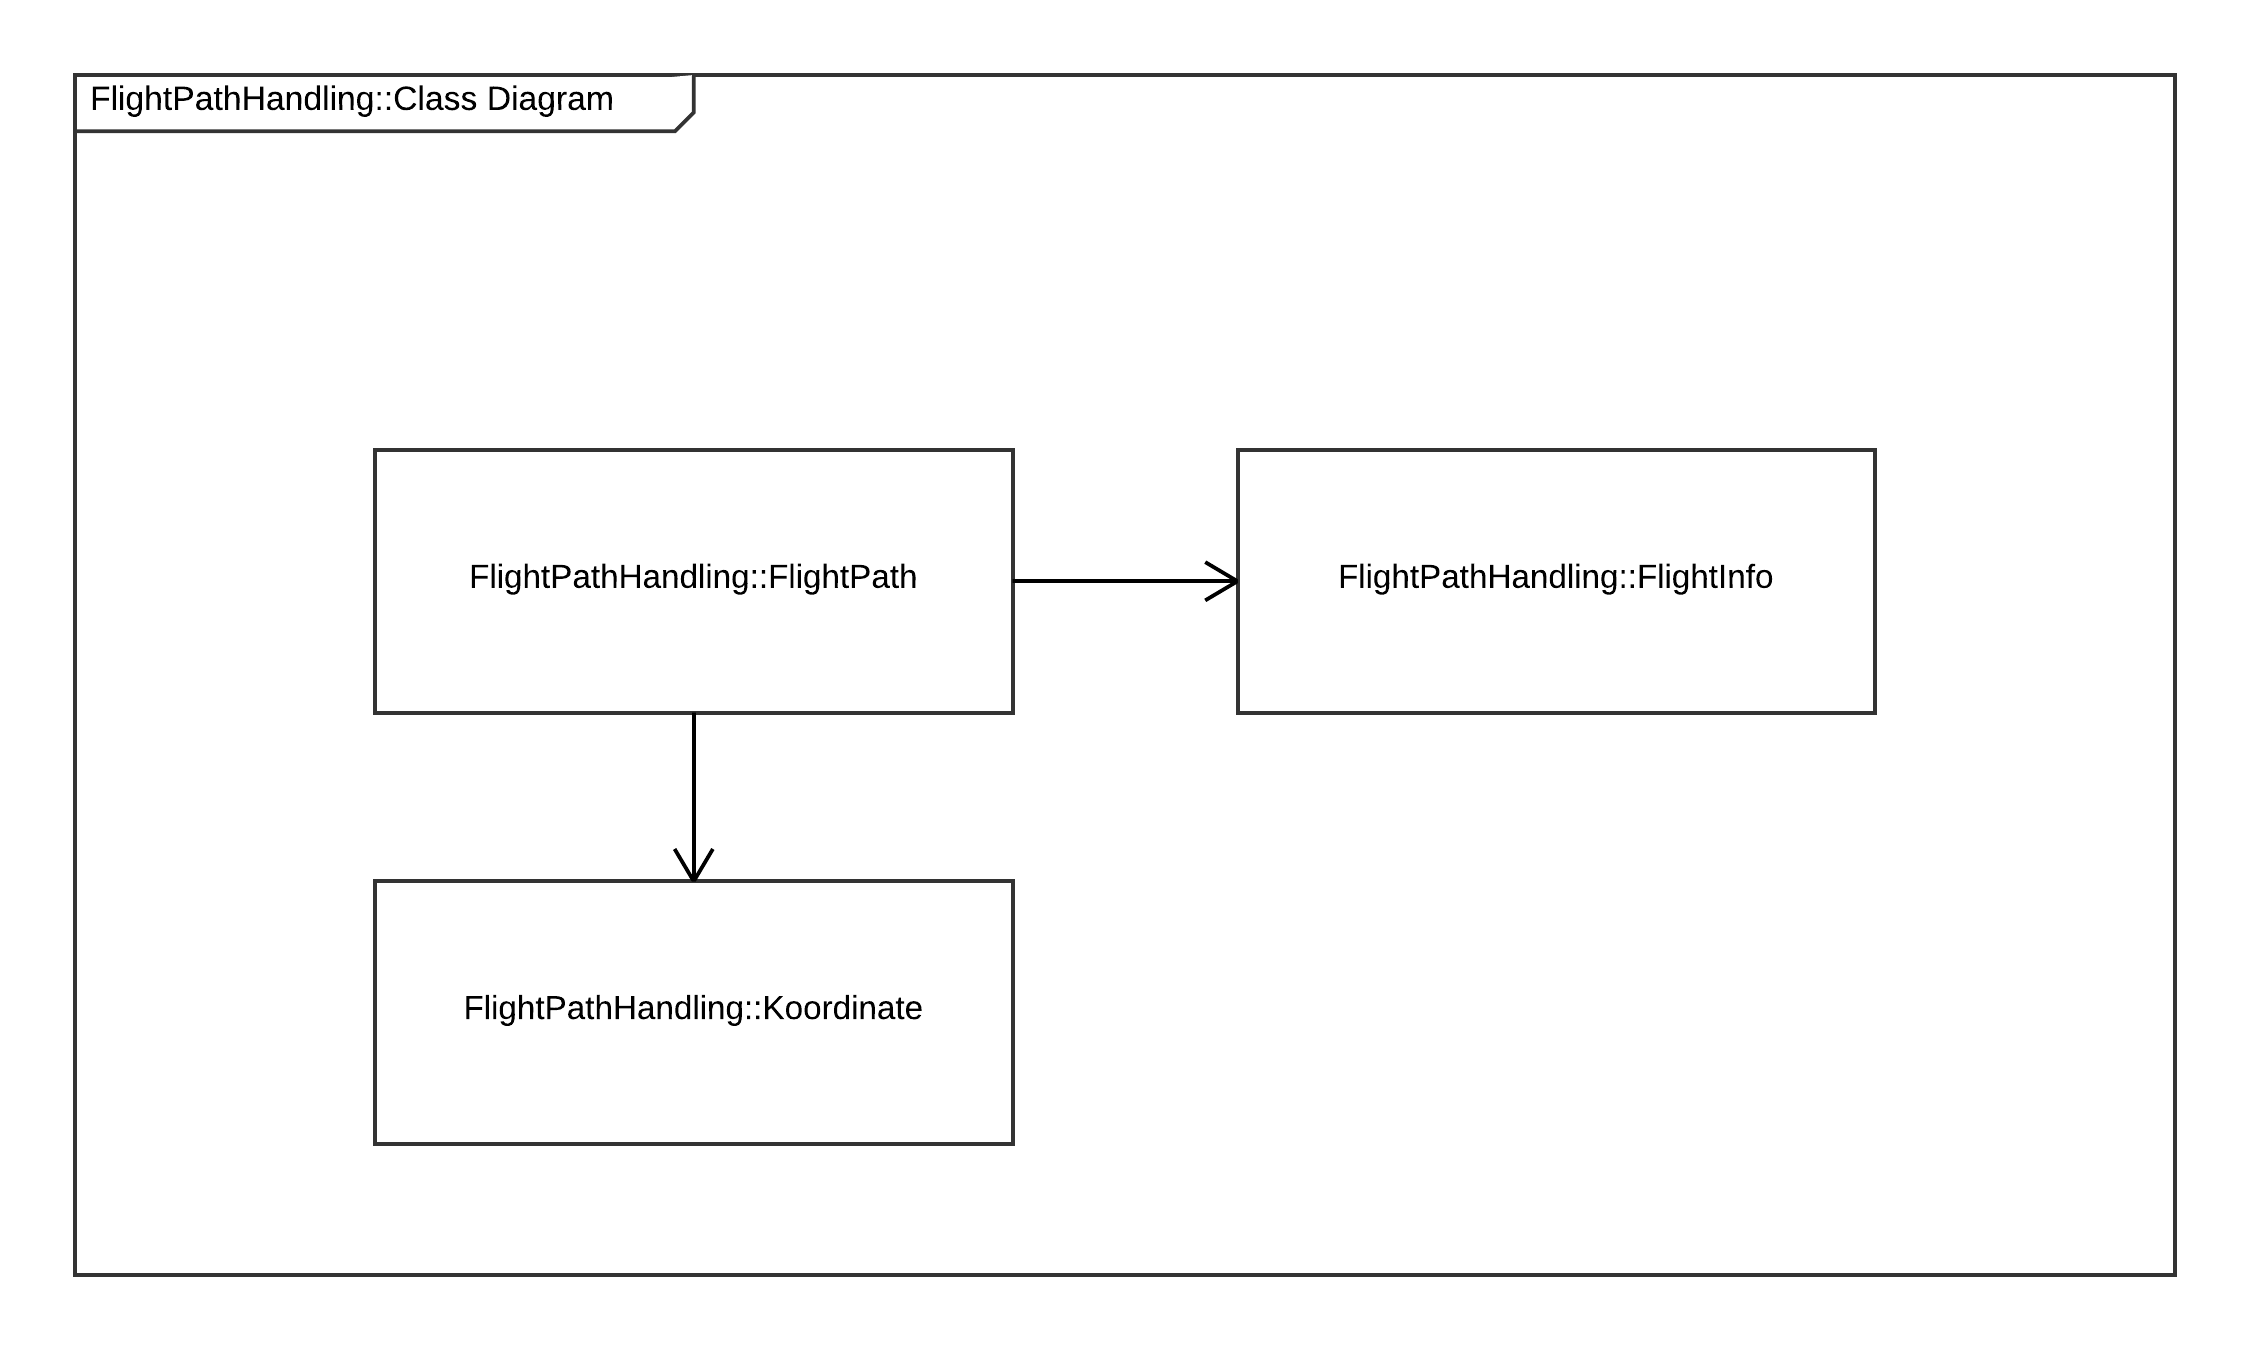
\includegraphics[width=0.7\textwidth]{Billeder/klasse_diagrammer/FlightPathHandlingDiagram.png}
	\vspace{-5pt}
	\caption{FlightPathHandling klasse diagram}
	\label{fig:FlightPathHandling_klasse_diagram}
\end{figure}

\textbf{FlightPath}\\
Klassen FlightPath bruger både FlightInfo og Coordinate klasserne til at udgøre en FlightPath.

\textbf{Coordinate}\\
Coordinate klassen håndtere det GPS koordinater som brugeren ønsker dronen skal flyve til.

\textbf{FlightInfo}\\
FlightInfo klassen håndtere data om ruten så som flyvehøjde, dato for flyvning.

\textbf{FileHandling}\\
FileHandling klassen genere en fil ud fra data'en i FlightPath som så sendes til dronen.

\textbf{JSONFormat}\\
Klassen nedarver fra FileHandling for at kunne bruges som FileHandling. Klassen genere en JSON fil som kan sendes til dronen.

\newpage
\subsection{UserHandling}
Klasse diagrammet viser hvilket klasser som udgør UserHandling pakken som vist på figur \ref{fig:pakke_diagram}.

\vspace{-5pt}
%kommentar
\begin{figure}[H]
	\centering
	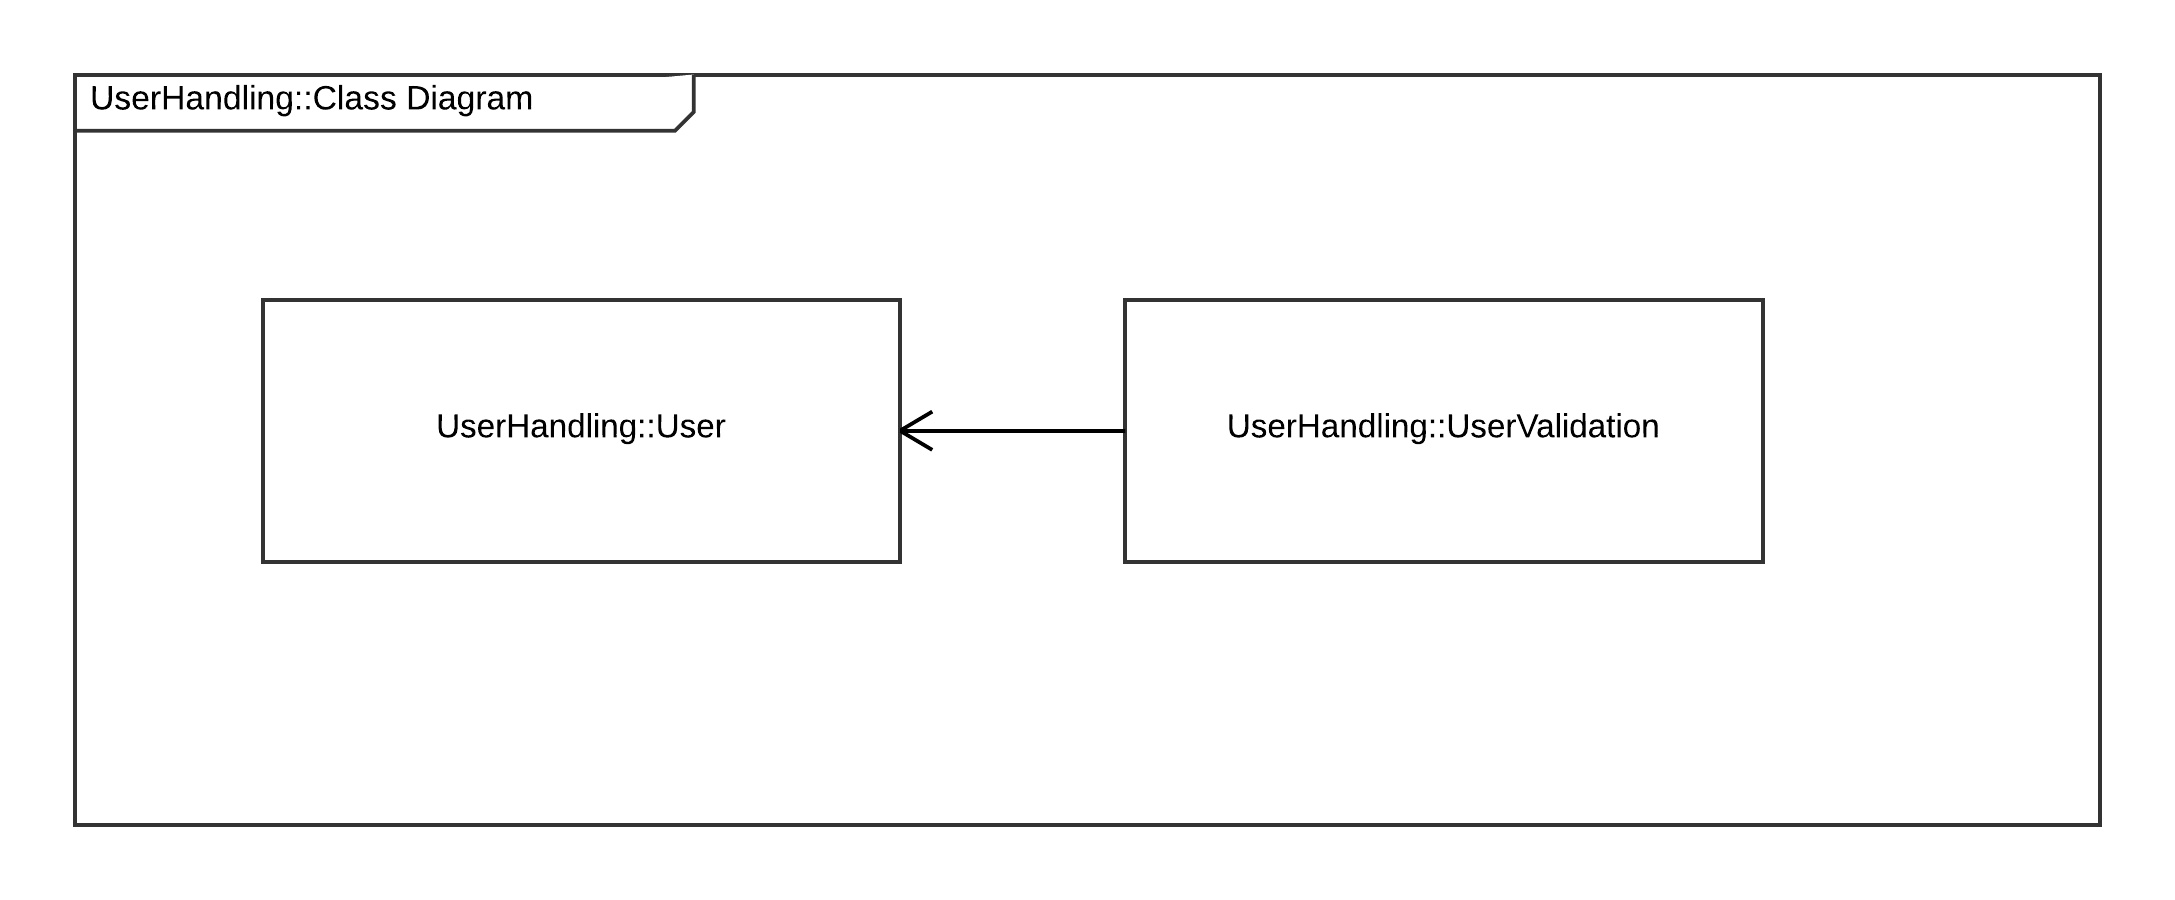
\includegraphics[width=0.7\textwidth]{Billeder/klasse_diagrammer/UserHandlingDiagram.png}
	\vspace{-5pt}
	\caption{UserHandling klasse diagram}
	\label{fig:UserHandling_klasse_diagram}
\end{figure}

\textbf{User}\\
User klassen indeholder alle data om brugerne i systemet. Klassen bliver også brugt af UserValidation i forbindelse med login/log out.

\textbf{UserValidation}\\
UserValidation klassen har ansvaret for at validere en user når der bliver forsøgt login.\\

\newpage
\subsection{DatabaseHandling}
Klasse diagrammet viser hvilket klasser som udgør DatabaseHandling pakken som vist på figur \ref{fig:pakke_diagram}.

\vspace{-5pt}
%kommentar
\begin{figure}[H]
	\centering
	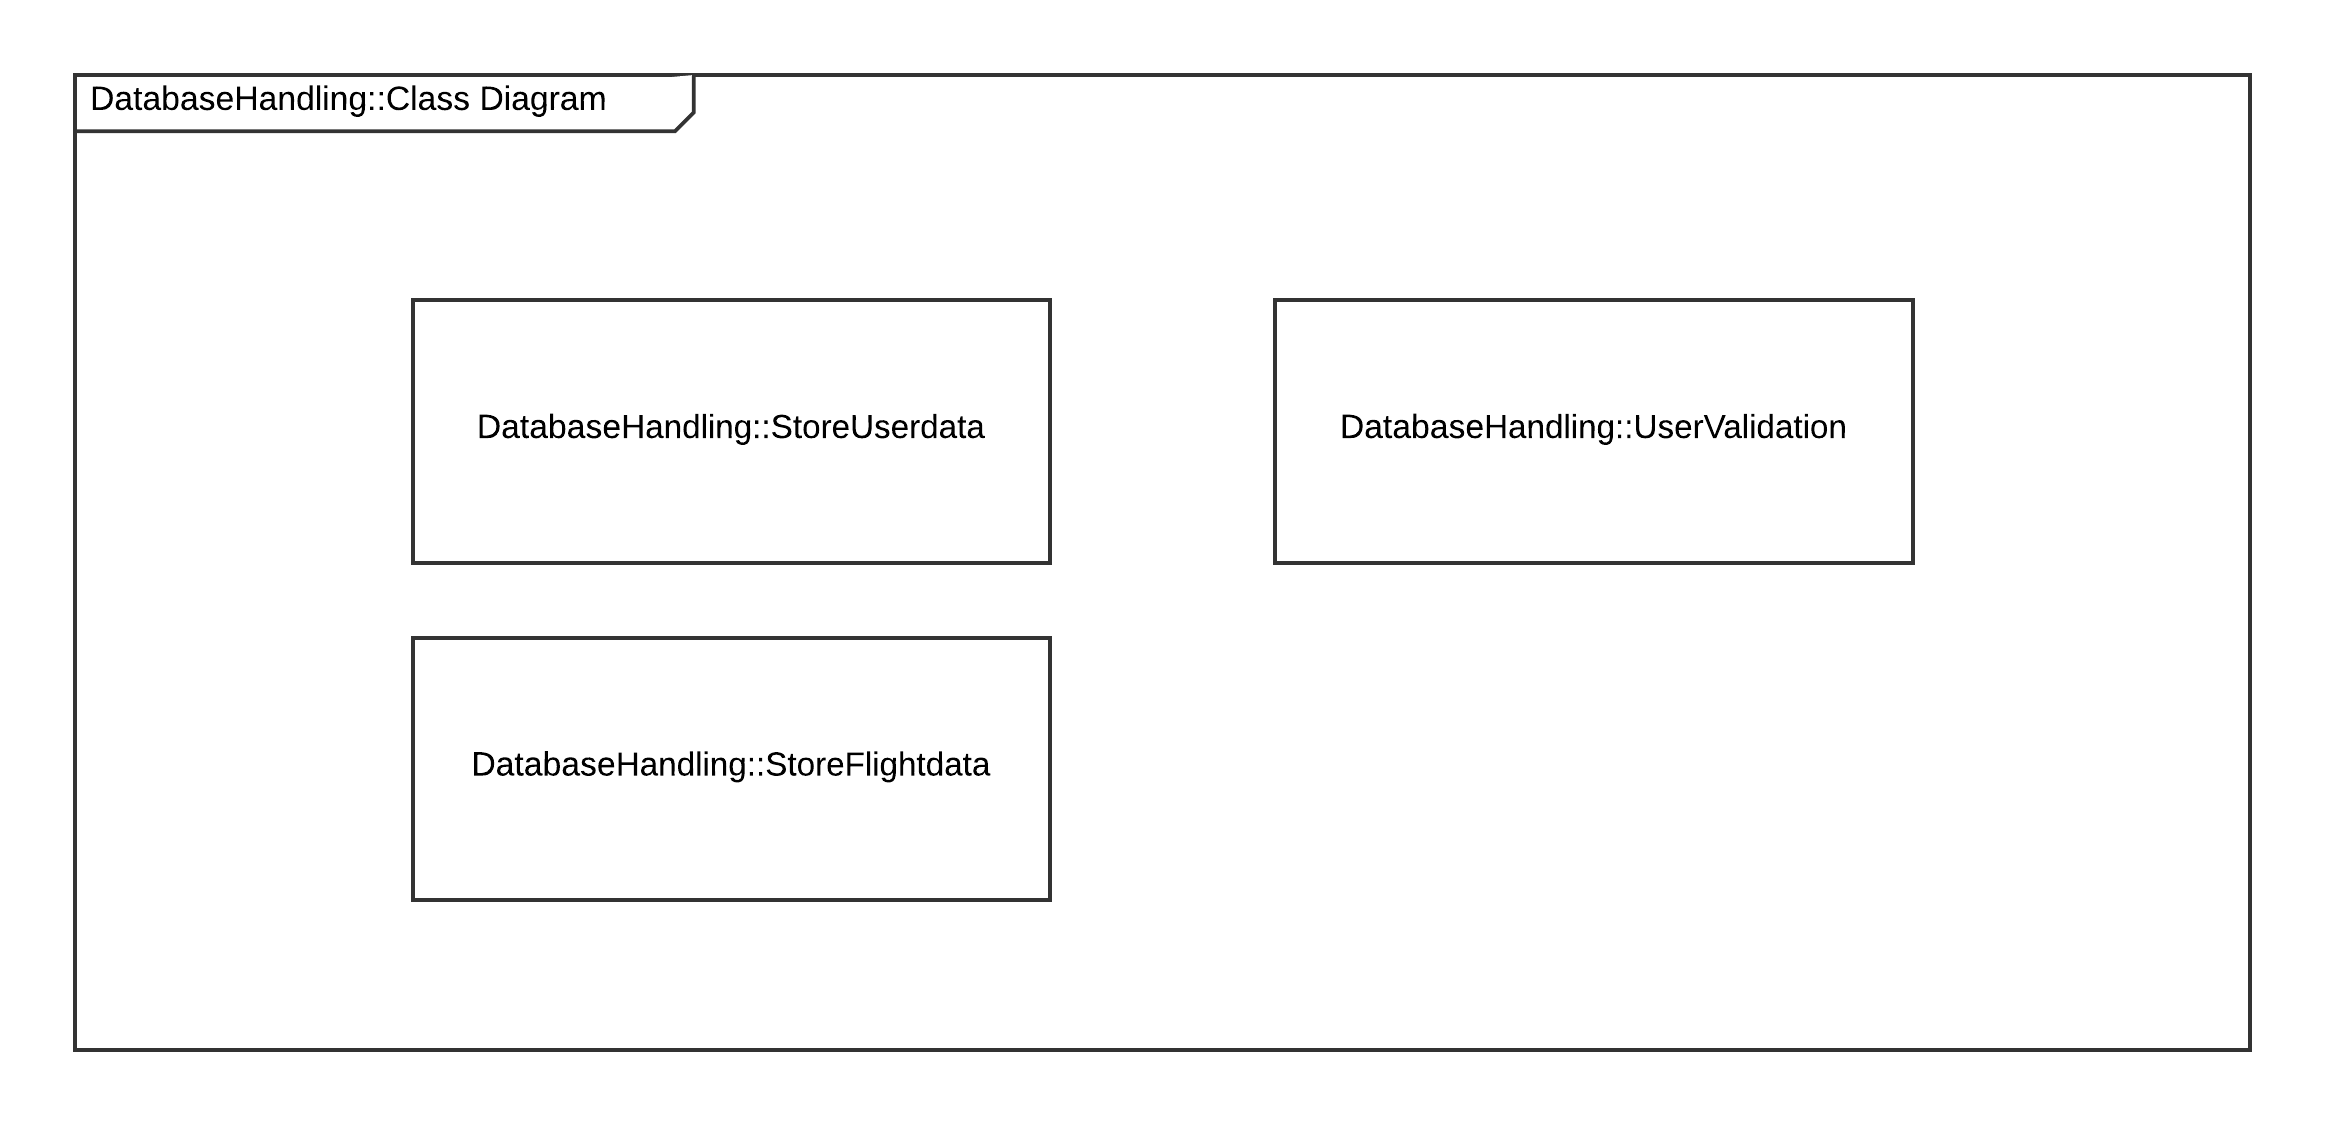
\includegraphics[width=0.7\textwidth]{Billeder/klasse_diagrammer/DatabaseHandling.png}
	\vspace{-5pt}
	\caption{DatabaseHandling klasse diagram}
	\label{fig:DatabaseHandling_klasse_diagram}
\end{figure}

\textbf{DatabaseConnection}\\
Superklassen DatabaseConnection har til ansvar at skabe forbindelse til databasen og lukke kommunikationen ned efter data overførelse. De andre klasser nedarver fra klassen så de kan oprette forbindelse og lukke forbindelsen.

\textbf{StoreUserdata}\\
Klassen opdatere brugerdata i databasen. Igennem nedarvningen fra superklassen DatabaseConnection kan StoreUserdata også oprette forbindelse og lukke forbindelsen igen til databasen.

\textbf{StoreFlightdata}\\
StoreFlightdata gemmer alle data omkring flyvning. Denne klasse bruges løbende under flyvning når billeder bliver modtaget og skal gemmes til en igangværende flyvning.

\textbf{UserValidation}\\
UserValidation validaere bruger ved forsøg på login og giver adgang til systemet hvis brugeren er valid.

\newpage
\subsection{CommunicationHandling}
Klasse diagrammet viser hvilket klasser som udgør CommunicationHandling pakken som vist på figur \ref{fig:pakke_diagram}.

\vspace{-5pt}
%kommentar
\begin{figure}[H]
	\centering
	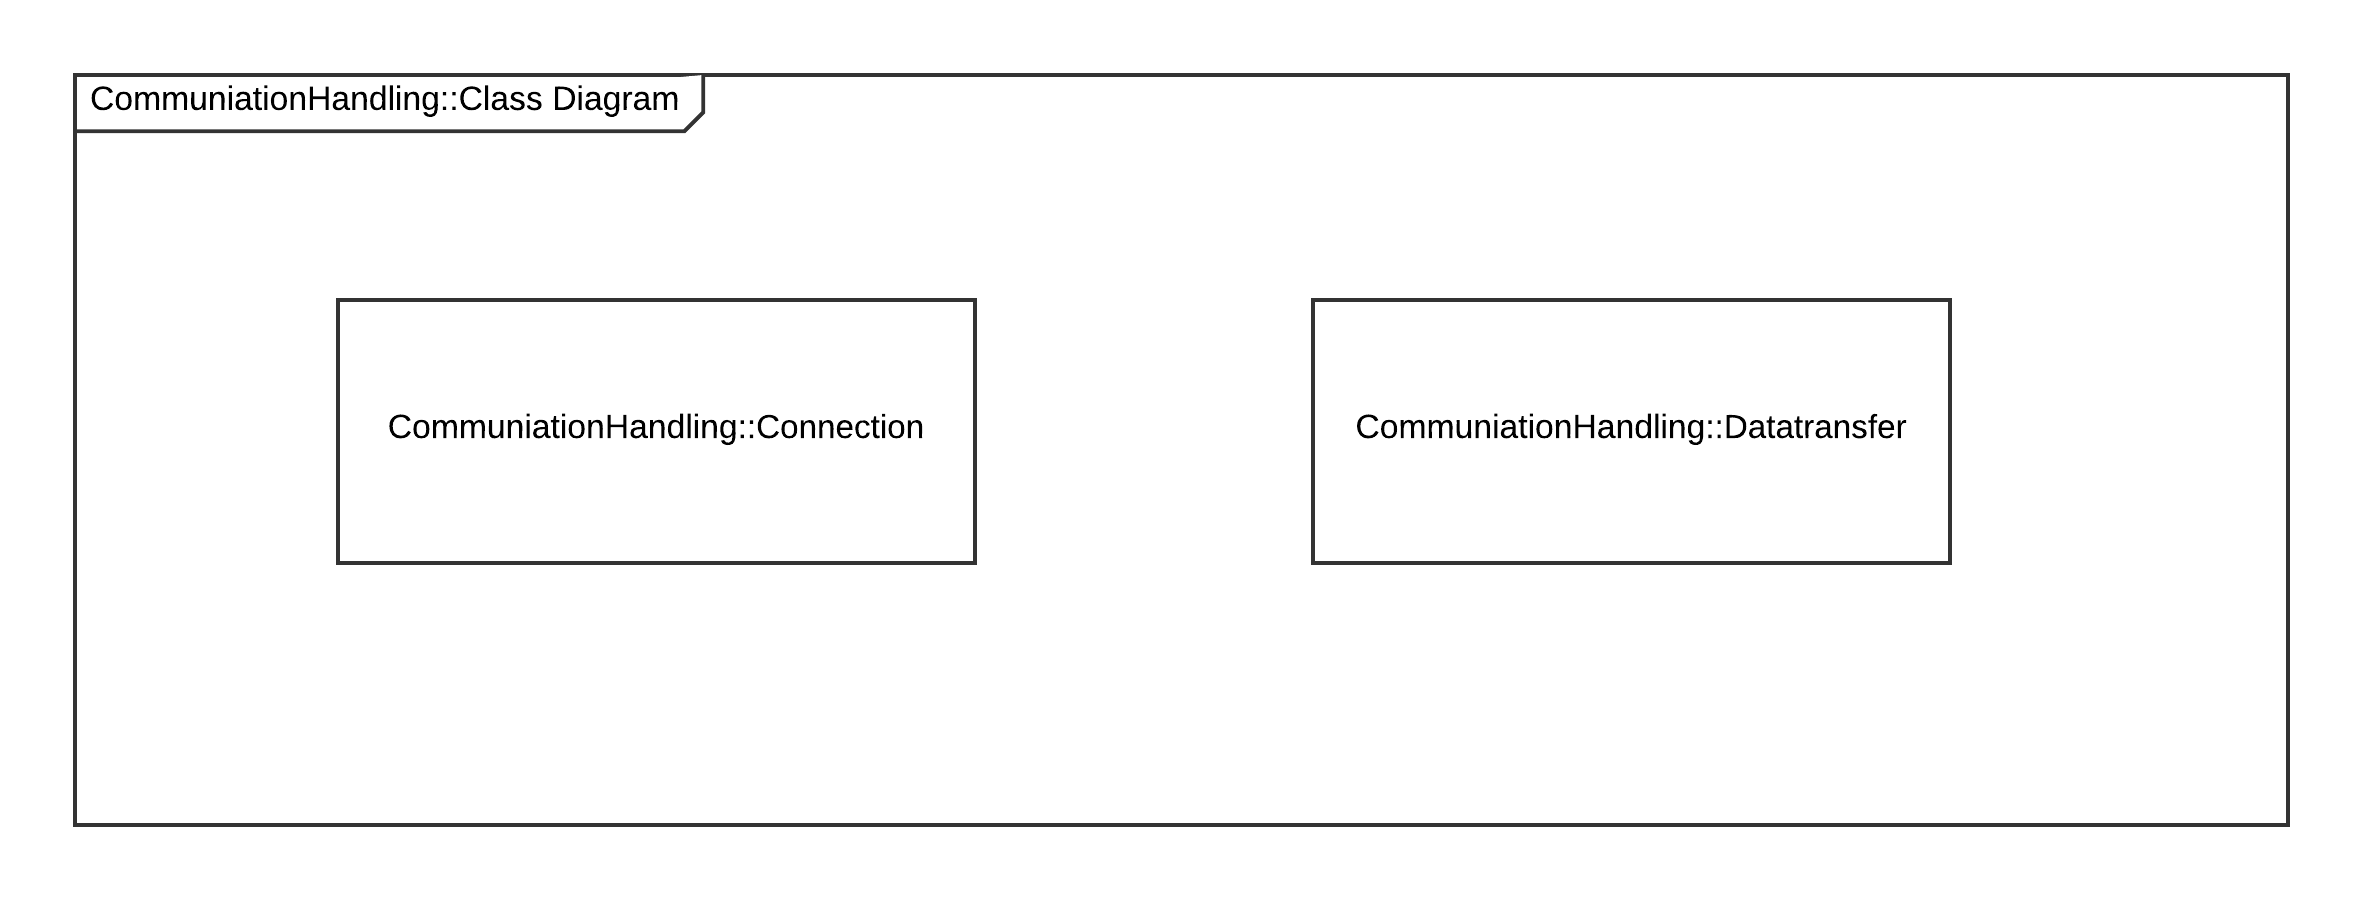
\includegraphics[width=0.7\textwidth]{Billeder/klasse_diagrammer/CommunicationHandling.png}
	\vspace{-5pt}
	\caption{CommunicationHandling klasse diagram}
	\label{fig:CommunicationHandling_klasse_diagram}
\end{figure}

\textbf{Connection}\\
Connection klassen har til ansvar for at skabe forbindelse imellem serveren og dronen.

\textbf{Datatransfer}\\
Datatransfer klassen bruger connection klassen til at oprette forbindelse til dronen inden data'en sendes. 
